\documentclass{article}
% Change "article" to "report" to get rid of page number on title page
\usepackage{amsmath,amsfonts,amsthm,amssymb}
\usepackage{setspace}
\usepackage{Tabbing}
\usepackage{fancyhdr}
\usepackage{lastpage}
\usepackage{extramarks}
\usepackage{chngpage}
\usepackage{soul,color}
\usepackage{graphicx,float,wrapfig}
\usepackage{listings}

% In case you need to adjust margins:
\topmargin=-0.45in      %
\evensidemargin=0in     %
\oddsidemargin=0in      %
\textwidth=6.5in        %
\textheight=9.0in       %
\headsep=0.25in         %

% Homework Specific Information
\newcommand{\hmwkTitle}{Homework 4}
\newcommand{\hmwkDueDate}{Apr 4, 2013}
\newcommand{\hmwkClass}{Bayesian Statistical Methods}
\newcommand{\hmwkClassTime}{}
\newcommand{\hmwkClassInstructor}{}
\newcommand{\hmwkAuthorName}{Andrew Kurzawski}

% Setup the header and footer
\pagestyle{fancy}                                                       %
\lhead{\hmwkAuthorName}                                                 %
\chead{\hmwkClass\ (\hmwkClassInstructor\ \hmwkClassTime): \hmwkTitle}  %
\rhead{\firstxmark}                                                     %
\lfoot{\lastxmark}                                                      %
\cfoot{}                                                                %
\rfoot{Page\ \thepage\ of\ \pageref{LastPage}}                          %
\renewcommand\headrulewidth{0.4pt}                                      %
\renewcommand\footrulewidth{0.4pt}                                      %

% This is used to trace down (pin point) problems
% in latexing a document:
%\tracingall

%%%%%%%%%%%%%%%%%%%%%%%%%%%%%%%%%%%%%%%%%%%%%%%%%%%%%%%%%%%%%
% Some tools
\newcommand{\enterProblemHeader}[1]{\nobreak\extramarks{#1}{#1 continued on next page\ldots}\nobreak%
                                    \nobreak\extramarks{#1 (continued)}{#1 continued on next page\ldots}\nobreak}%
\newcommand{\exitProblemHeader}[1]{\nobreak\extramarks{#1 (continued)}{#1 continued on next page\ldots}\nobreak%
                                   \nobreak\extramarks{#1}{}\nobreak}%

\newlength{\labelLength}
\newcommand{\labelAnswer}[2]
  {\settowidth{\labelLength}{#1}%
   \addtolength{\labelLength}{0.25in}%
   \changetext{}{-\labelLength}{}{}{}%
   \noindent\fbox{\begin{minipage}[c]{\columnwidth}#2\end{minipage}}%
   \marginpar{\fbox{#1}}%

   % We put the blank space above in order to make sure this
   % \marginpar gets correctly placed.
   \changetext{}{+\labelLength}{}{}{}}%

\setcounter{secnumdepth}{0}
\newcommand{\homeworkProblemName}{}%
\newcounter{homeworkProblemCounter}%
\newenvironment{homeworkProblem}[1][Problem \arabic{homeworkProblemCounter}]%
  {\stepcounter{homeworkProblemCounter}%
   \renewcommand{\homeworkProblemName}{#1}%
   \section{\homeworkProblemName}%
   \enterProblemHeader{\homeworkProblemName}}%
  {\exitProblemHeader{\homeworkProblemName}}%

\newcommand{\problemAnswer}[1]
  {\noindent\fbox{\begin{minipage}[c]{\columnwidth}#1\end{minipage}}}%

\newcommand{\problemLAnswer}[1]
  {\labelAnswer{\homeworkProblemName}{#1}}

\newcommand{\homeworkSectionName}{}%
\newlength{\homeworkSectionLabelLength}{}%
\newenvironment{homeworkSection}[1]%
  {% We put this space here to make sure we're not connected to the above.
   % Otherwise the changetext can do funny things to the other margin

   \renewcommand{\homeworkSectionName}{#1}%
   \settowidth{\homeworkSectionLabelLength}{\homeworkSectionName}%
   \addtolength{\homeworkSectionLabelLength}{0.25in}%
   \changetext{}{-\homeworkSectionLabelLength}{}{}{}%
   \subsection{\homeworkSectionName}%
   \enterProblemHeader{\homeworkProblemName\ [\homeworkSectionName]}}%
  {\enterProblemHeader{\homeworkProblemName}%

   % We put the blank space above in order to make sure this margin
   % change doesn't happen too soon (otherwise \sectionAnswer's can
   % get ugly about their \marginpar placement.
   \changetext{}{+\homeworkSectionLabelLength}{}{}{}}%

\newcommand{\sectionAnswer}[1]
  {% We put this space here to make sure we're disconnected from the previous
   % passage

   \noindent\fbox{\begin{minipage}[c]{\columnwidth}#1\end{minipage}}%
   \enterProblemHeader{\homeworkProblemName}\exitProblemHeader{\homeworkProblemName}%
   \marginpar{\fbox{\homeworkSectionName}}%

   % We put the blank space above in order to make sure this
   % \marginpar gets correctly placed.
   }%

% Python Setup
\lstset{
  language=Python,
  showstringspaces=false,
  formfeed=\newpage,
  tabsize=4,
  commentstyle=\itshape,
  basicstyle=\ttfamily,
  morekeywords={models, lambda, forms}
}

% Uncomment lines and make changes to have a header
\newcommand{\code}[1]{ % change to [2]
  % \hrulefill
  % \subsection*{#1}
  \lstinputlisting{#1} % change to {#2}
  \vspace{2em}
}

%%%%%%%%%%%%%%%%%%%%%%%%%%%%%%%%%%%%%%%%%%%%%%%%%%%%%%%%%%%%%


%%%%%%%%%%%%%%%%%%%%%%%%%%%%%%%%%%%%%%%%%%%%%%%%%%%%%%%%%%%%%
% Make title
\title{\vspace{2in}\textmd{\textbf{\hmwkClass:\ \hmwkTitle}}\\\normalsize\vspace{0.1in}\small{Due\ on\ \hmwkDueDate}\\\vspace{0.1in}\large{\textit{\hmwkClassInstructor\ \hmwkClassTime}}\vspace{3in}}
\date{}
\author{\textbf{\hmwkAuthorName}}
%%%%%%%%%%%%%%%%%%%%%%%%%%%%%%%%%%%%%%%%%%%%%%%%%%%%%%%%%%%%%

\begin{document}
\begin{spacing}{1.1}
\maketitle
\newpage
% Uncomment the \tableofcontents and \newpage lines to get a Contents page
% Uncomment the \setcounter line as well if you do NOT want subsections
%       listed in Contents
%\setcounter{tocdepth}{1}
%\tableofcontents
%\newpage

% When problems are long, it may be desirable to put a \newpage or a
% \clearpage before each homeworkProblem environment

\clearpage

\begin{homeworkProblem}

Low birth weight risk factors using binary regression.

\subsection{Part A}
Without any prior knowledge of the problem, I chose to use disperse normal priors ($\mu = 0$ and $\tau = 10^{-6}$) for the regression coefficients.

\subsection{Part B}
Table~\ref{tab:mods_1} lists the regression parameters and DICs for five different models.

\begin{table}[h!]
\caption{Problem 1 model variants}
\begin{center}
  \begin{tabular}{cccccc}
    \hline\noalign{\smallskip}
    Model Number & Age & Weight & Race & Visits & DIC \\
    \noalign{\smallskip}\hline\noalign{\smallskip}
    1 & X & X & X & X & 235.73 \\
    2 & X & X & X & & 233.59 \\
    3 & & X & X & & 231.91 \\
    4 & & X & & & 232.80 \\
    5 & X & X & & & 233.04 \\
    \noalign{\smallskip}\hline
  \end{tabular}
\end{center}
\label{tab:mods_1}
\end{table}

\subsection{Part C}
Based on the DIC of model 3 compared to the other models, it appears that weight and race are the most significant covariates. We can justify the exclusion of age and number of visits by examining the 95\% confidence intervals of all four variables in model 1. In Table~\ref{tab:conf}, we can see that the parameters most likely to be zero are age and number of visits.

\begin{table}[h!]
\caption{Model 1 confidence intervals}
\begin{center}
  \begin{tabular}{ccc}
    \hline\noalign{\smallskip}
    Variable & 2.5 & 97.5 \\
    \noalign{\smallskip}\hline\noalign{\smallskip}
    Intercept & -1.266 & 3.393 \\
    Age & -0.091 & 0.043 \\
    Weight & -0.024 & 0. \\
    Race & -0.106 & 0.55 \\
    Visits & -0.352 & 0.278 \\
    \noalign{\smallskip}\hline
  \end{tabular}
\end{center}
\label{tab:conf}
\end{table}

\end{homeworkProblem}



\begin{homeworkProblem}

Hierarchical models: impact on beta-blockers on mortality.

\subsection{Part A} 
Fit the model. See $\tau^2$ output in Figure~\ref{fig:tau_2a}.

\begin{figure}[h!]
\begin{center}
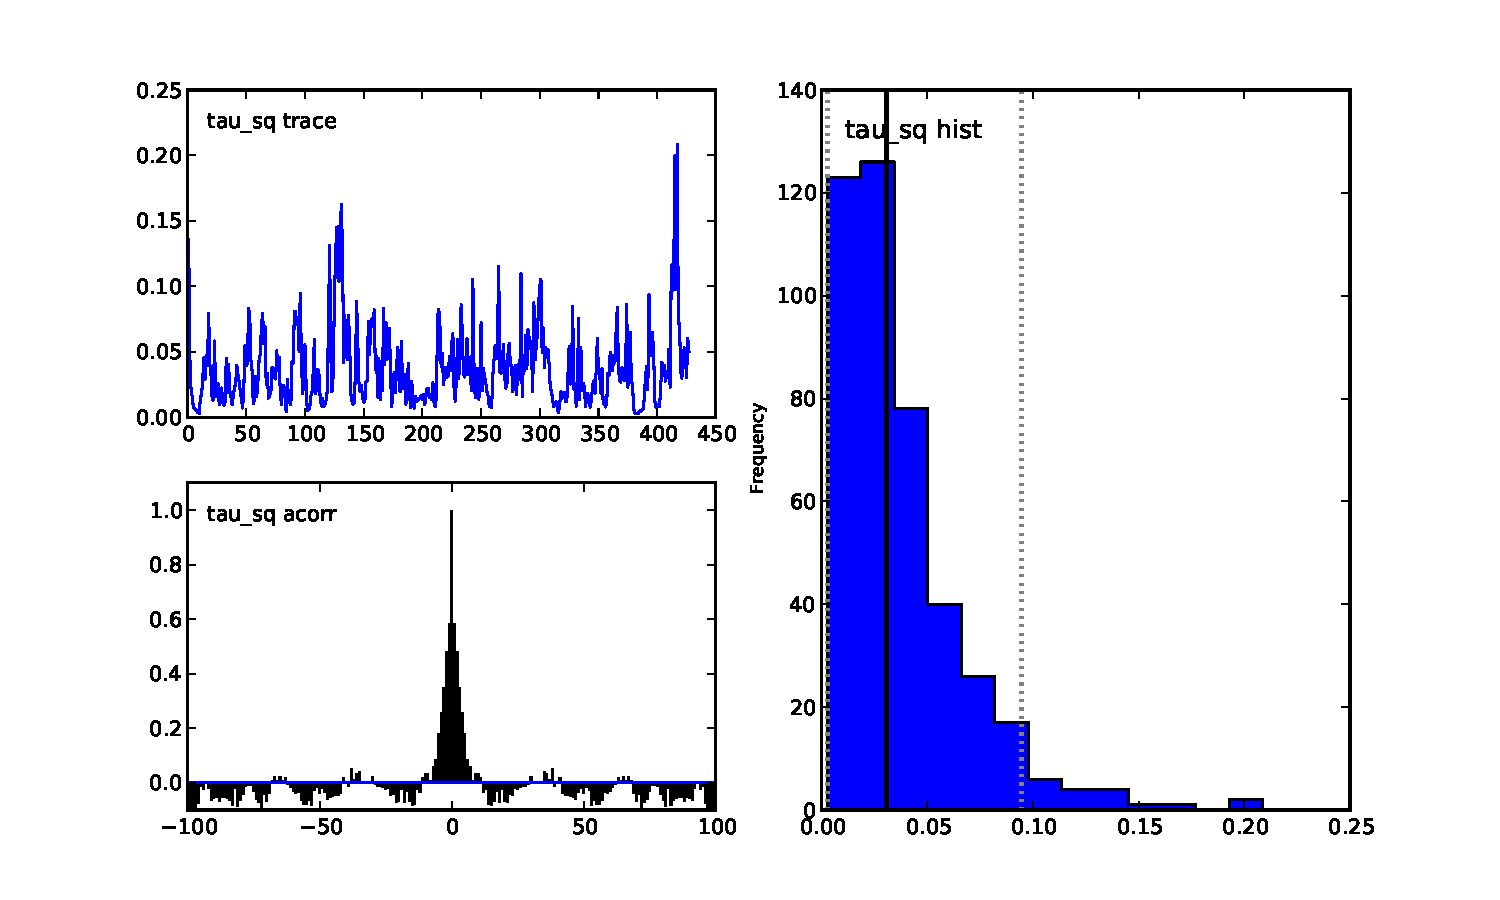
\includegraphics[height=3.0in]{./Figures/Report/tau_sq_2a.pdf}
\end{center}
\caption{Trace, autocorrelation, and histogram of $\tau^2$ for fitted model}
\label{fig:tau_2a}
\end{figure}

Model:
\code{./Code/2a.py}

\subsection{Part B}

We can judge the effectiveness of beta-blockers by examining the predicted values of the overall log odds ratio,$\theta$, and the between model variance, $\tau^2$. The posterior mean of $\theta$ is positive (around 0.25) indicating that the odds of surviving a heart attack when given beta blockers is greater than the survival odds of the control group. However, there is a lot of heterogeneity between studies as evidnet by the raw log odds ratios, $y_j$, and noticing that six of the studies have negative values indicating better survival in the control group. Additionally, the predicted mean of $\tau$ is 0.195 which is on the same order as $\theta$ indicating high variability between studies.  

\subsection{Part C}

The posterior means of $\theta_j$ were all positive and clustered closer to the overall mean ($\theta$), while the raw estimates were occasionally negitive and had larger variation.

\subsection{Part D}

Incomplete.  \\

Model:
\code{./Code/2d.py}

\subsection{Part E}

Currently, the model treats every patient in the study the same. To reduce heterogeneity, patients could be binned by age, weight, etc., to assess the effect of beta blockers in different subsets of the population.

\end{homeworkProblem}



\begin{homeworkProblem}

We know that the posterior hyperparameters of the Beta-Binomial Model are

\begin{equation}
\hat{\alpha} = \delta m_i + \bar{y},\quad \hat{\beta} = \delta(1-m_i) + n - \bar{y}
\label{post_hyp}
\end{equation}

\noindent and the expected value of the posterior distribution is

\begin{equation}
E[\theta_i | \delta,m,y] = \frac{\hat{\alpha}}{\hat{\alpha} + \hat{\beta}}
\label{post_exp_1}
\end{equation}

This simplifies to

\begin{equation}
E[\theta_i | \delta,m,y] = \frac{\delta m_i + \bar{y}}{\delta + n}
\label{post_exp_2}
\end{equation}

The shrinkage factor on $\delta$ is

\begin{equation}
\frac{\delta}{\delta + n}
\label{sfac}
\end{equation}

Putting a uniform (0,1) prior on this results in

\begin{equation}
p\left(\frac{\delta}{\delta + n}\right) = 1
\label{sfac_prob}
\end{equation}

Transformation of variables:

\begin{equation}
x = \frac{\delta}{\delta + n}
\label{sfac_tran1}
\end{equation}

\begin{equation}
p(\delta) = f\left(\frac{\delta}{\delta + n}\right) \frac{dx}{d\delta}
\label{sfac_tran2}
\end{equation}

\noindent where

\begin{equation}
f\left(\frac{\delta}{\delta + n}\right) = 1
\label{sfac_tran3}
\end{equation}

\noindent so that leaves

\begin{equation}
p(\delta) = \frac{n}{(n+\delta)^2}
\label{delt_prob}
\end{equation}


\end{homeworkProblem}



\begin{homeworkProblem}

Gibbs sampling algorithm for a normal-normal model.

Step 1: Pick initial values for $\mu$ and $\tau^2$.

Step 2: Sample $\mu_i$ from its full conditional.

Step 3: Sample $\mu$ from its full conditional using the new value of $\mu_i$.

Step 4: Sample $\tau^2$ from its full conditional using the new values of $\mu_i$ and $\mu$.

Step 5: Repeat 2-4 using updated values of $\mu_i$, $\mu$, and $\tau^2$ at each step. \\
 
In order to do this, we must assign priors to $\mu$ and $\tau^2$, derive the posterior probability $p(\mu_i,\mu,\tau^2|y,\sigma^2)$, and derive the full conditionals for $\mu_i$, $\mu$, and $\tau^2$. See the attached graph paper for details.

\end{homeworkProblem}


\end{spacing}
\end{document}

%%%%%%%%%%%%%%%%%%%%%%%%%%%%%%%%%%%%%%%%%%%%%%%%%%%%%%%%%%%%%

%----------------------------------------------------------------------%
% The following is copyright and licensing information for
% redistribution of this LaTeX source code; it also includes a liability
% statement. If this source code is not being redistributed to others,
% it may be omitted. It has no effect on the function of the above code.
%----------------------------------------------------------------------%
% Copyright (c) 2007, 2008, 2009, 2010, 2011 by Theodore P. Pavlic
%
% Unless otherwise expressly stated, this work is licensed under the
% Creative Commons Attribution-Noncommercial 3.0 United States License. To
% view a copy of this license, visit
% http://creativecommons.org/licenses/by-nc/3.0/us/ or send a letter to
% Creative Commons, 171 Second Street, Suite 300, San Francisco,
% California, 94105, USA.
%
% THE SOFTWARE IS PROVIDED "AS IS", WITHOUT WARRANTY OF ANY KIND, EXPRESS
% OR IMPLIED, INCLUDING BUT NOT LIMITED TO THE WARRANTIES OF
% MERCHANTABILITY, FITNESS FOR A PARTICULAR PURPOSE AND NONINFRINGEMENT.
% IN NO EVENT SHALL THE AUTHORS OR COPYRIGHT HOLDERS BE LIABLE FOR ANY
% CLAIM, DAMAGES OR OTHER LIABILITY, WHETHER IN AN ACTION OF CONTRACT,
% TORT OR OTHERWISE, ARISING FROM, OUT OF OR IN CONNECTION WITH THE
% SOFTWARE OR THE USE OR OTHER DEALINGS IN THE SOFTWARE.
%----------------------------------------------------------------------%